% Generated by pysimcount.pfboundratio -- do not edit; regenerate instead.
% figure: bound-ratio-lie-trotter -- Lie-Trotter S1: Trotter number from each bound / measured r, against n
% metric=r_ratio gatebase=cz; geometric mean over seeds [1, 2, 3, 4, 5, 6, 7, 8, 9, 10], bars min-max; r_method=measured (denominator); bounds: Analytic bound, Minimised bound, Commutator bound (2018), Commutator bound (2021), Empirical fit (2018)
% sizes: np-main n = [4, 5, 6, 7, 8, 10]; np-main-n9 n = [9]; np-main-n11 n = [11]
% run set np-main-n9 made from uncommitted code (git_dirty), accepted: run at e42ff29 with the only modified tracked file pysimcount/pfseeds.py (an aggregation module the run does not import); checked with git diff --stat e42ff29 -- pysimcount/ on 2026-11-08
% run set np-main-n11 made from uncommitted code (git_dirty), accepted: run at e42ff29 with the only modified tracked file pysimcount/pfseeds.py (an aggregation module the run does not import); checked with git diff --stat e42ff29 -- pysimcount/ on 2026-11-08
% formulas: Lie-Trotter S1
% figure made at git_commit=e5d9ee696f892e28aced765585653760f8a427c4 git_dirty=False
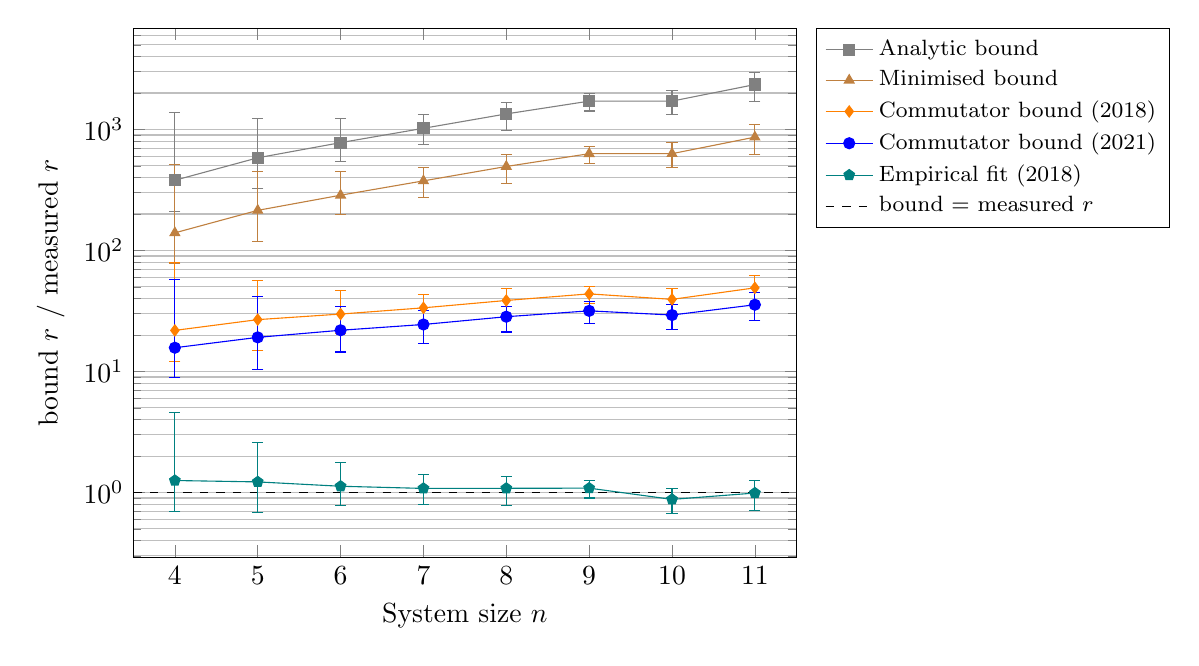
\begin{tikzpicture}
  \begin{semilogyaxis}[
    width=10cm, height=8.3cm,
    xlabel={System size $n$}, ylabel={bound $r$ / measured $r$},
    xmin=3.5, xmax=11.5,
    xtick={4,5,6,7,8,9,10,11},
    ymajorgrids=true, yminorgrids=true,
    legend pos=outer north east, legend cell align=left,
    legend style={font=\footnotesize},
  ]
    \addplot[dashed, black, domain=3.5:11.5, samples=2, forget plot] {1};
    \addplot[solid, gray, mark=square*, mark size=2pt, error bars/.cd, y dir=both, y explicit] coordinates {
      (4,380.201) -= (0,168.651) += (0,1008.78)
      (5,583.211) -= (0,259.529) += (0,643.45)
      (6,778.209) -= (0,236.699) += (0,445.018)
      (7,1022.25) -= (0,272.215) += (0,300.549)
      (8,1344.07) -= (0,366.779) += (0,338.129)
      (9,1714.12) -= (0,293.639) += (0,266.677)
      (10,1714.98) -= (0,395.034) += (0,389.853)
      (11,2349.19) -= (0,650.21) += (0,617.554)
    };
    \addlegendentry{Analytic bound}
    \addplot[solid, brown, mark=triangle*, mark size=2pt, error bars/.cd, y dir=both, y explicit] coordinates {
      (4,139.87) -= (0,62.0442) += (0,371.116)
      (5,214.554) -= (0,95.4765) += (0,236.714)
      (6,286.289) -= (0,87.0775) += (0,163.714)
      (7,376.066) -= (0,100.143) += (0,110.566)
      (8,494.459) -= (0,134.931) += (0,124.391)
      (9,630.593) -= (0,108.024) += (0,98.1054)
      (10,630.906) -= (0,145.325) += (0,143.419)
      (11,864.222) -= (0,239.199) += (0,227.186)
    };
    \addlegendentry{Minimised bound}
    \addplot[solid, orange, mark=diamond*, mark size=2pt, error bars/.cd, y dir=both, y explicit] coordinates {
      (4,21.8591) -= (0,9.69634) += (0,57.9983)
      (5,26.8247) -= (0,11.937) += (0,29.5953)
      (6,29.8279) -= (0,9.07244) += (0,17.0571)
      (7,33.5843) -= (0,8.9432) += (0,9.87404)
      (8,38.6377) -= (0,10.5437) += (0,9.72009)
      (9,43.8004) -= (0,7.50324) += (0,6.81431)
      (10,39.44) -= (0,9.08474) += (0,8.96558)
      (11,49.1139) -= (0,13.5937) += (0,12.911)
    };
    \addlegendentry{Commutator bound (2018)}
    \addplot[solid, blue, mark=oplus*, mark size=2pt, error bars/.cd, y dir=both, y explicit] coordinates {
      (4,15.7164) -= (0,6.85956) += (0,42.0713)
      (5,19.1472) -= (0,8.67721) += (0,22.4584)
      (6,21.9132) -= (0,7.43173) += (0,12.5606)
      (7,24.4605) -= (0,7.47308) += (0,7.21698)
      (8,28.3543) -= (0,7.14192) += (0,6.34438)
      (9,31.7037) -= (0,6.72755) += (0,6.0103)
      (10,29.2721) -= (0,7.04405) += (0,6.61907)
      (11,35.6115) -= (0,9.25393) += (0,9.51505)
    };
    \addlegendentry{Commutator bound (2021)}
    \addplot[solid, teal, mark=pentagon*, mark size=2pt, error bars/.cd, y dir=both, y explicit] coordinates {
      (4,1.25642) -= (0,0.557329) += (0,3.33365)
      (5,1.22359) -= (0,0.544497) += (0,1.34997)
      (6,1.12641) -= (0,0.342609) += (0,0.644138)
      (7,1.08107) -= (0,0.287878) += (0,0.317842)
      (8,1.08304) -= (0,0.295548) += (0,0.272461)
      (9,1.08673) -= (0,0.186162) += (0,0.169069)
      (10,0.877352) -= (0,0.202092) += (0,0.199442)
      (11,0.989826) -= (0,0.273964) += (0,0.260205)
    };
    \addlegendentry{Empirical fit (2018)}
    \addlegendimage{dashed, black}
    \addlegendentry{bound $=$ measured $r$}
  \end{semilogyaxis}
\end{tikzpicture}
